\documentclass{article}
\usepackage{geometry} % Set margins
\usepackage{setspace} % For double spacing
\usepackage{titlesec} % For section formatting
\usepackage{enumitem} % For list formatting
\usepackage{xcolor} % For highlighting text
\usepackage{amssymb,tabu,placeins,algorithmic} % natbib
\usepackage{mathtools,bm}
\usepackage[ruled,vlined,linesnumbered]{algorithm2e}
\usepackage{hyperref}
\usepackage{lipsum}
\usepackage{graphicx}
\usepackage[style=authoryear]{biblatex}
\addbibresource{kderm.bib}

\renewcommand*{\finalnamedelim}{\addspace\&\space}
\renewcommand*{\finallistdelim}{\addspace\&\space}
\renewcommand*{\multicitedelim}{\addsemicolon\space}
\renewcommand*{\nameyeardelim}{\addcomma\space}


% Set page margins
\geometry{
    left=1in,
    right=1in,
    top=1in,
    bottom=1in
}

% Set section formatting
\titleformat{\section}
{\bfseries\Large}
{\thesection.}
{0.5em}
{}

% Set list formatting
\setlist{noitemsep}

% Set double spacing
\doublespacing
\setlength{\parskip}{1em}

% Define colors for highlighting
\definecolor{myblue}{RGB}{0,0,200}
\definecolor{myblack}{RGB}{0, 0, 0}

% Color algorithm
\newenvironment{algocolor}{%
   \setlength{\parindent}{0pt}
   \itshape
   \color{myblue}
}{}

\date{\vspace{-8ex}}

\begin{document}


\title{Response to Reviewer 1's \\ \textit{"Report on 'Distortion corrected kernel density estimation on Riemannian manifolds” by F.Cheng, R.J Hyndman \& A.Panagiotelis'} }
% \author{}
% \date{}

\maketitle

We would like to extend our appreciation to the reviewer for their detailed and insightful feedback on our manuscript titled "Distortion corrected kernel density estimator on Riemannian manifolds." Your comments have been invaluable in enhancing the clarity and depth of our work. We have carefully addressed each point raised and provide detailed responses below highlighted in blue text.

\section*{Review}

\textit{However, I believe that the quality of the paper could be improved by comparing in more detail the performances with other density estimation methods that do not rely on a first step being the estimation of an embedding. Indeed, while embedding and then correcting for the distortion is a good idea, if one is only interested in estimating the density then the additional embedding step may potentially introduce unnecessary bias/instability. I have detailed my points below.}

1. \textit{In page 2 lines \(20-27\) it is said that several methods for density estimation on manifolds are limited to the case of known manifolds. While this is true for most of the examples, this is not true for [2. In this example the manifold needs not to be known for the method to be tractable. However it is assumed that the observations are living in a small tubular neighbourhood around the manifold, not exactly on it. Furthermore, at this point in the paper it would be sensible to cite the works of Berenfeld \& Hoffman [1] (which is actually mentioned later on) and Divol [3]. These works show that several types of KDEs are actually minimax optimal in the context of density estimation on manifolds. The goal of the present being slightly different (estimating the density of the sample after embedding), the comparison with the aforementioned works would be relevant and would help the reader to understand the contribution of the present paper.}

   \textcolor{blue}{We have revised the manuscript to clarify the distinction between our approach and those that do not require a known manifold. Additionally, we have included citations to the works of \cite{berenfeld2021-den} and \cite{divol2022measure} to provide context on minimax optimality in density estimation on manifolds. In the introduction we now state:\\
   ``Recently, \cite{berenfeld2021-den}, \cite{berenfeld2022-est} and \cite{divol2022measure} demonstrated the minimax optimality of certain types of KDE on manifolds. In contrast, our objective in this paper is to propose a new KDE for data that lie on some unknown manifold found using embedding techniques.''
   }

2. \textit{Following the previous remark, when the data is embedded in a Euclidean space (such as in the simulated examples: twin peaks and the semihypersphere), it is possible (even if the manifold is unknown) to perform density estimation directly on the data (and not after estimating an embedding) with, for instance, KDEs [1, 3] or special Dirichlet process mixtures [2] while preserving optimal statistical convergence properties (at least theoretically). Would your (empirical) results stay competitive in this case?}

   \textcolor{blue}{While it is possible to perform KDE on the data without using an embedding, this is challenging for the high dimensional examples we consider. The popular \texttt{ks} package [\cite{Duong2007-up}] in R recommends that it not be used for dimensions greater than 6 due to issues with numerical instability. The \texttt{weird} package [\cite{hyndman2024-weird}] in R also implements multivariate kernel density estimation, however its function to find the bandwidth matrix was prohibitively slow even for a dimension of 5. The example we consider is 100-dimensional. In this case, we have coded a KDE by hand with a bandwidth proportional to an identity matrix, i.e. $\mathbf{H} = h^2 \mathbf{I}$. The scale factor $h$ is found using Silverman's rule adapted for multivariate data : $h = \left(\frac{4}{d+2}\right)^{\frac{1}{d+4}} n^{-\frac{1}{d+4}}$. In our semi-hypersphere example, $d=100$ and $n=10,000$. Note that due to the curse of dimensionality the KDE on 100-dimensional data is somewhat flat with the densities of all points close to zero. This can be shown by observing the distribution of the estimated densities evaluated at each observation. This bottom panel (yellow violin plot) of Figure \ref{fig:kde} shows the results for a 100-dimensional KDE without dimension reduction. In contrast to the true densities and the KDEs on emeddings, the 100-dimensional KDE estimate does not detect the high proportion of points with relatively lower densities.}
 
   \begin{figure}[!h]
   	\begin{center}
    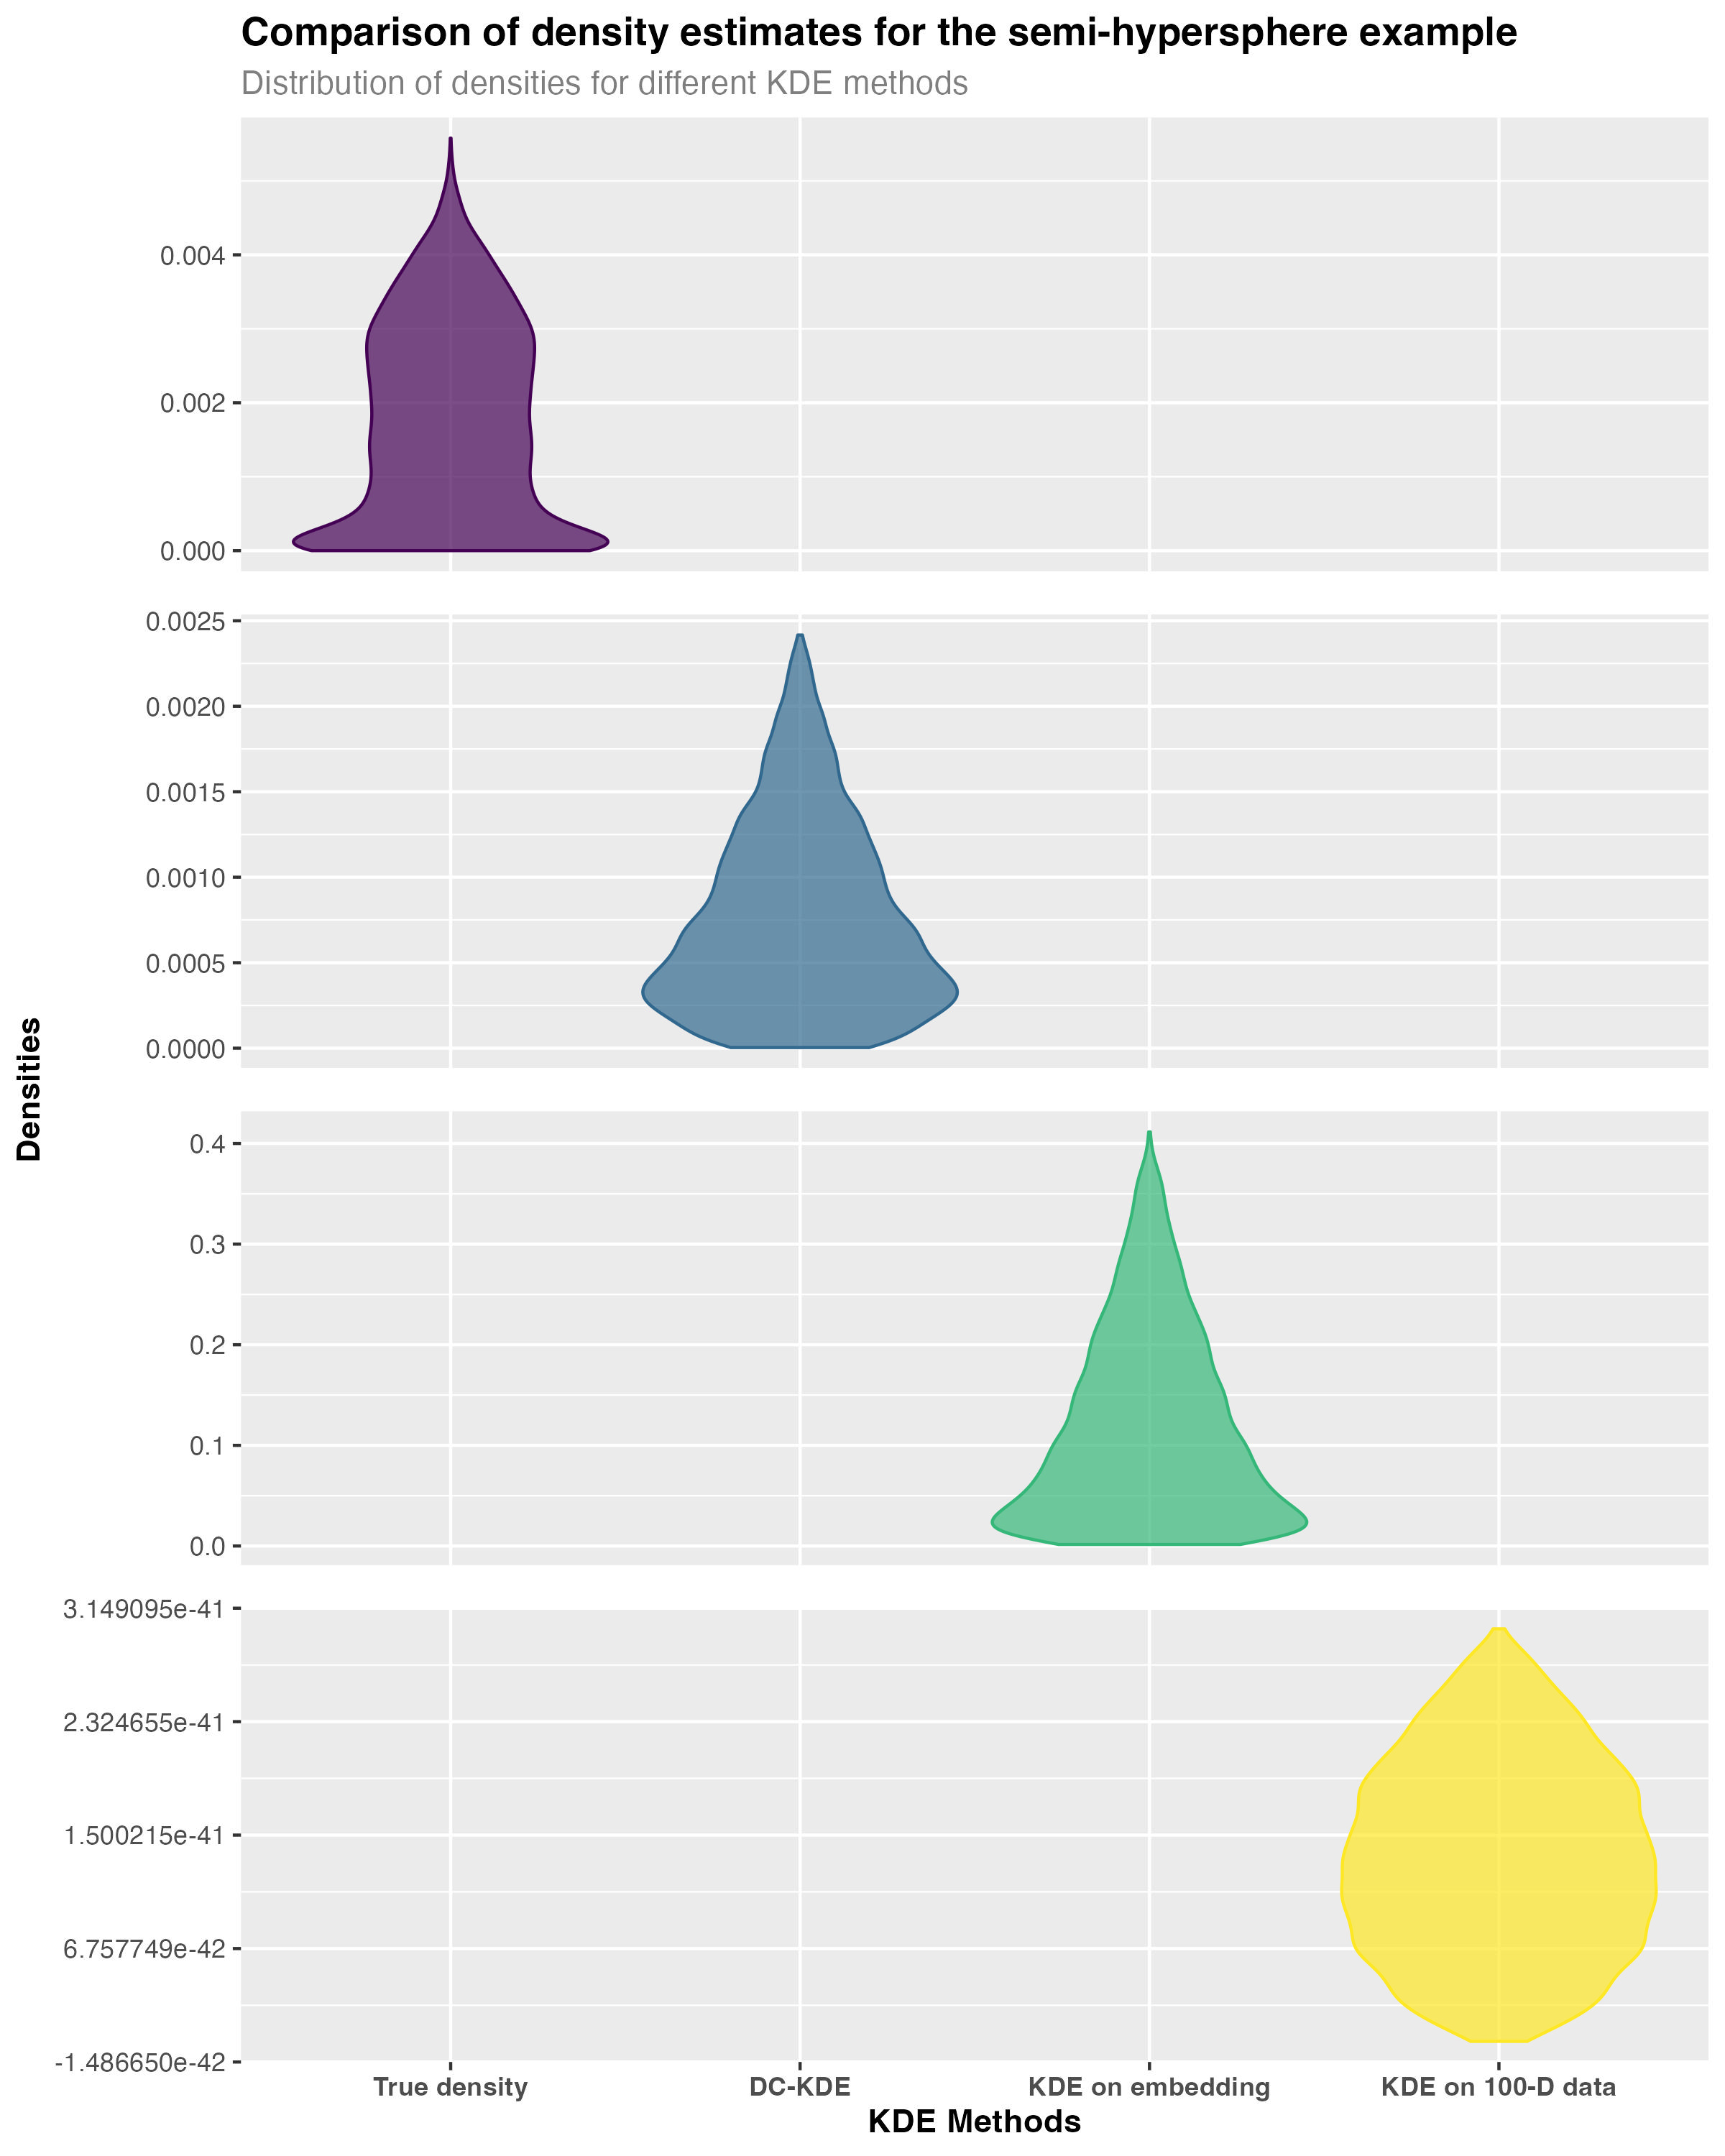
\includegraphics[width=0.4\linewidth]{kde_compare_violin.jpeg}\end{center}
    \caption{Comparison of KDE methods for high-dimensional data.}
    \label{fig:kde}
    \end{figure}

   \textcolor{blue}{
   %Figure \ref{fig:kde} shows the comparison of the density estimates for the 100-D example with different density estimations. We use different violin plots to display the distribution of the density estimates, and they are, from left to right, the true density of the manifold, distortion-corrected KDE, KDE using ISOMAP embedding, and KDE on the 100-D data with $\mathbf{H} = h^2 \mathbf{I}$ as bandwidth matrix. By comparing with the true density distribution, both in the violin shape and the y-axis scale, we could tell that DC-KDE gives the closest density estimates to the true ones, and KDE on 100-D data performs very poorly with almost all 0 estimates. \\
   In high-dimensional spaces, the data sparsity leads to exponentially slower convergence rates and requires an impractically large sample size to achieve reliable density estimates. Computationally, bandwidth selection algorithms are extremely demanding, both in terms of processing time and memory requirements. All these factors combined make traditional KDE methods unsuitable for 100-dimensional data, and dimension reduction is essential as proposed here.
   }

3. \textit{During all of the experiments (both with simulated and real data), the choices of the parameters \(\varepsilon, r\) are not really discussed thoroughly, even though it is known that tuning them is usually quite hard. The problem for \(r\) is even not related to the manifold learning problem as it also appears in classical KDE on flat Euclidean spaces. I believe it would be beneficial to give some guidance on this matter or at least some observations.}

   \textcolor{blue}{We acknowledge the importance of parameter tuning and have added more details on this. Regarding the choice of \(\varepsilon\) we use as stated at the end of Section 2.2 the default choice of 0.4. Experimenting with alternative values did not lead to appreciably better results that the default choice, and we now state this clearly in the paper. Regarding the scale $r$ we similarly experimented with different values. Since there is only a single parameter this could be tuned with reference to the downstream task. For example, for anomaly detection, $r$ could be chosen to maximise the coherence between selecting anomalies both in and out of sample using cross validation. We have revised the manuscript to state this in final paragraph of the conclusion.
   }

\section*{Miscellaneous}

1. \textit{page 2 line 32: it should be made clear at this point that the dimension \(d\) is either considered known or needs to be estimated separately (i.e., the proposed method is not directly dimension agnostic).}

   \textcolor{blue}{
   We have clarified that the dimension \(d\) is assumed to be known as a priori or estimated separately, as our method is not dimension agnostic and $d$ is a crucial parameter. In the second paragraph of the paper we state (with the part in bold now added):\\
  ``These algorithms, which include ISOMAP, LLE, t-SNE, and UMAP among others, can be thought of as a mapping \(\psi:M\rightarrow \mathbb{R}^d\) that take points on the manifold \(\bm{p}\) to \(d\)-dimensional vectors \(\bm{y}\), \textbf{where the dimension $d$ is either assumed to be known a priori or needs to be estimated separately}.'' }

2. \textit{Equation (1): a reference to a relevant textbook/source for the formula would be useful for the inexperienced reader.}

   \textcolor{blue}{A book reference, Chapter 3 of "Riemannian Geometry" by \cite{doCarmo1992-rm}, has been added to guide readers to a relevant source for Equation (1). \\
   ``By a change of variables, this would imply the following density for \(\bm{y}\),
\begin{equation}
\label{eq:changevar}
Pr(\bm{y}\in\psi(\mathcal{A}))=\int\limits_{\psi(\mathcal{A})} (f\circ\psi^{-1})(\bm{y})|\det \bm{H}(\bm{y})|^{1/2}d\bm{y},
\end{equation}
where \(\psi(\mathcal{A})\) is the image of \(\mathcal{A}\) under \(\psi\) and \(\bm{H}(\bm{y})\) is the Riemannian metric expressed in local coordinates given by the mapping \(\psi\) \autocite{doCarmo1992-rm}.''
   }

3. \textit{page 3 line 24: I think the author meant to write "Riemannian metric."}

   \textcolor{blue}{%
   We have corrected the missing "metric" in the specified line. \\
   ``Critical to our estimator, is obtaining an estimate of $|\bm{H}(\bm{y})|^{1/2}$ for this purpose we use the Learn Metric algorithm of \cite{Perrault-Joncas2013-pq} which augments any dimension reduction algorithm with an estimate of the Riemannian \textbf{metric} at each data point.''
   }

4. \textit{page 3 line 38: it is not clear how a 2 or 3-dimensional is constructed and is actually confusing in the context: is \(d=2\) or \(3?\) probably not but clarifications would be useful here.}

   \textcolor{blue}{
   Clarifications have been added to explain the construction of 2 or 3-dimensional spaces in order to visualize the output of dimension reduction, where \(d=2\) for a 2-dimensional scatterplot and \(d=3\) for a 3-dimensional scatterplot. We now state: \\
  ``In terms of data visualization, our approach allows a two or three-dimensional scatterplot of \(\bm{y}\) to be augmented by coloring points according to the magnitude of the density estimate, where the dimension of \(\bm{y}\), \(d\), is set as 2 or 3 in the dimension reduction algorithms."
   }

5. \textit{page 7 lines \(36-42\): this is a bit confusing, at first the graph is described as being a k-NN graph but later a radius parameter is mentioned (which is usually a parameter used to define random geometric graphs, not k-NN ones). It would be beneficial to clarify this point/the construction of the graph.}

   \textcolor{blue}{
   Thank you for pointing this out. Either a K-nearest neighbor (KNN) or fixed radius method could be used. In the Learn Metric algorithm, the weighted neighborhood graph is constructed by using a fixed-radius nearest neighbor search instead of a KNN approach. The fixed-radius method considers all points within a specified radius of \(\sqrt{\epsilon}\). This radius parameter allows the graph to adapt to varying densities in the data, capturing local structure more effectively. By using a fixed-radius approach, the algorithm ensures that the graph reflects the underlying geometry of the data manifold, which is crucial for the analysis. We now clarify this: \\
   ``First, a weighted neighborhood graph is constructed, with edges between \(\bm{p}_i\) and \(\bm{p}_j\) when \(\bm{p}_i\) is a fixed-radius nearest neighbor of \(\bm{p}_j\) or vice versa, and edge weights depending on the distance between \(\bm{p}_i\) and \(\bm{p}_j\) on the manifold. The fixed-radius method considers all points within a specified radius of \(\sqrt{\varepsilon}\), allowing the graph to adapt to varying densities in the data and to capture local structure more effectively. Second, the discrete Laplacian on this graph \(\hat{\mathcal{L}}_{\varepsilon,n}\) is estimated \autocite{Zhou2011-za}, where \(\sqrt{\varepsilon}\) is the radius parameter in the previous step and a constant value $c=0.25$ is used for the use of heat kernel in the weighted neighborhood graph.''
   }

6. \textit{page 9 /algorithm 1: at step 2 it looks like you are using the symmetric normalized graph Laplacian. Shouldn't it be \(\tilde{W}=D^{-1 / 2} W D^{-1 / 2}\) and not \(D^{-1} W D^{-1}\)? Also, the constant \(c\) in the definition of \(\tilde{\mathcal{L}}_{n, \varepsilon}\) is not defined, does the value matter?}

   \textcolor{blue}{Here we simply restate the algorithm as defined in Algorithm 1 of \cite{Perrault-Joncas2013-pq} who define \(\tilde{W}=D^{-\lambda} W D^{- \lambda}\), and then $\lambda=1$ in Step 2 of their Algorithm 3. We agree that by setting $\lambda=1/2$, we would be using the symmetric normalized graph Laplacian but for consistency with the original reference, set \(\tilde{W}=D^{-1} W D^{-1)} \) and use this in our computation. \\
   % We have corrected the definition of the symmetric normalized graph Laplacian and provided an explanation for the constant \(c\) in the definition of \(\tilde{\mathcal{L}}_{n, \varepsilon}\). \\
   Setting \(c=0.25\) is recommended when using heat kernel used in the weighted neighborhood graph $w_{i,j}=\exp(-\frac{1}{\varepsilon}\|\bm{x}_i-\bm{x}_j\|^2)$. The values for \(c\) is stated in Section 2.2, and we have provided an explanation for this choice now and included the value of \(c\) in Step 2 of Algorithm 1. We also note that since \(c\) and ${\varepsilon}$ only enter Algorithm 1 as a product, it is sufficient to tune only one of these parameters. This is now also discussed in the paper at the end of Section 2.2.
   }

7. \textit{page 9 /algorithm 1: it looks like the steps \(3 \& 4\) are completely independent. In general, in order to get an estimated embedding one can use techniques based on neighborhood/nearest neighbors graphs (like Laplacian Eigenmaps). If one does that and then uses the same graph to perform step 4 would your technique be "improved"? Have you tried that? A few words on this would be helpful.}

   \textcolor{blue}{Thanks for your suggestion. Yes, we did use the same nearest neighbor graph from Step 1 to get the estimated embedding. The computational efficiency is largely improved by doing this as the nearest neighbor searching is the most time-consuming step. For implementation, we used approximate nearest neighbor searching methods proposed in another paper \cite{Cheng2021-dh}. We have now added further explanation in Section 2.2. \\
  ``This algorithm is implemented in a Python library *megaman* (\cite{McQueen2016-xz}) although our own results are based on a re-implementation of the algorithm in \texttt{R}. For computational efficiency, approximate nearest neighbor searching methods are implemented to construct the neighborhood graph (\cite{Cheng2021-dh}, \cite{Perrault-Joncas2013-pq}), which are then used in both steps 1 and 3.''
   }

8. \textit{page 10 line 30: it is stated that for the estimation of the density at an unobserved point one can use "any smoothed average of nearest neighbors." Isn't there the same problem as in the original problem of density estimation at observed points? i.e., isn't there distortion issues as well when doing that?}

   \textcolor{blue}{The referee is correct to point this out. Indeed to prevent this distortion the average of nearest neighbors should be weighted by a term that depends on the the determinant of the Riemannian at each of the nearest neighbors. We now state explicitly in the paper:\\
   ``To account for distortion, this average should be weighted by the determinant of the Riemannian at each of the nearest neighbors.''}

9. \textit{page 13 line 53: can you point to a reference for the behavior of t-SNE in this context?}

   \textcolor{blue}{\autocite{cai2022-tsne} has been added here for discussion about the clustering behavior of t-SNE. t-SNE is designed to preserve local structure of the high-dimensional data very well, which means it emphasizes similarities between nearby points, which can lead to the formation of apparent clusters in the low-dimensional visualization. The paper mentions an ``early exaggeration'' stage in t-SNE that allows for easier movement of clusters in the early stages of the algorithm. This can contribute to the formation of spurious clusters.}

10. \textit{page 15 line 48: a definition/short reminder on ranks and their definition would be beneficial (possibly in appendix?).}

   \textcolor{blue}{
   Thanks for your suggestion. We have included a brief definition of density rank in the Appendix B for clarity. \\
   ``The density rank used in the paper is defined as the relative position or order of an item within a set from the lowest to the highest, based on its density value.''
   }

\section*{Conclusion}

\textit{We are enthusiastic about the method and believe this is a valuable contribution; the only major missing point being, in my opinion, a more complete comparison with other methods. I hope my remarks will help the authors to improve the quality of the paper.}

\vspace{0.5cm}

\textcolor{blue}{We are grateful for the reviewer's enthusiasm and constructive remarks. We have made the suggested improvements and believe they have significantly enhanced the quality of the paper. Thank you once again for your valuable feedback.}

% \bibliographystyle{plainnat}
% \bibliography{references}

\printbibliography

\end{document}
